% $Id: serverConfigPrefPage.tex 10532 2010-03-16 15:57:20Z alexandra $
% Local Variables:
% ispell-check-comments: nil
% Local IspellDict: american
% End:
% --------------------------------------------------------
% User documentation
% copyright by BREDEX GmbH 2004
% --------------------------------------------------------

\label{serverConfigPrefPage}
\index{Preferences!AUT Agent}
%\index{Preferences!JRE}
%\index{JRE!Preferences}
\index{AUT Agent!Preferences}
\index{Add!AUT Agent}
\index{AUT Agent!Add}
%\index{Add!JRE}
%\index{JRE!Add}

\begin{enumerate}
\item In the \gdagent{} preference page, you can add, edit and delete \gdagent{}s and port numbers. 
\bxtipp{The \gdagent preference page can also be accessed from the \gdaut{} configuration dialog which you can open from the \gdproject{} properties.}

%\item The preference page is set up so that the port number and JRE details are shown for the currently selected \gdagent. If you want to add, edit or delete port numbers or JRE details for an \gdagent{}, select the \gdagent{} host in the list of \gdagent{}s. 
%\item To add items here, enter the name, number or path in the relevant field and click \bxcaption{Add}. The item you have entered will appear in the list. 
%\item To edit items here, select the item you want to edit and change the details in the text field, then click \bxcaption{Change}. The modified item will appear in the list. 
%\item To delete items here, select the item you want to delete and click \bxcaption{Remove}. 
%\item Any changes you make in the \gdagent preferences are then available in the \gdaut{} configuration properties. 
\end{enumerate}




\begin{figure}[p]
\begin{center}
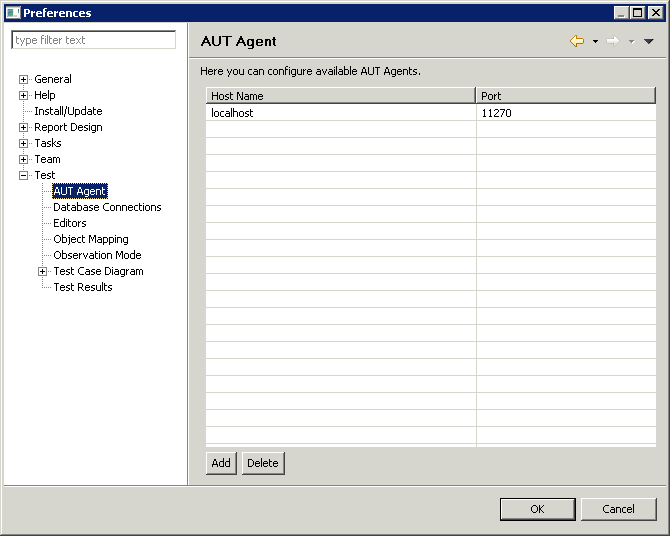
\includegraphics[width=12.5cm]{Tasks/Preferences/PS/serverconfig}
\caption{\gdagent Configuration Dialog}
\label{serverconfig}
\end{center}
\end{figure}







